\documentclass[oneside, 11pt]{article}

\usepackage[T1]{fontenc}
\usepackage[utf8]{inputenc}
\usepackage[english]{babel}

\usepackage{fouriernc}
\usepackage[detect-all, binary-units, separate-uncertainty=true,
            per-mode=symbol, retain-explicit-plus, retain-unity-mantissa=false]{siunitx}

\usepackage{setspace}
\setstretch{1.2}

\setlength{\parskip}{\smallskipamount}
\setlength{\parindent}{0pt}

\usepackage[headheight=14pt]{geometry}
\geometry{marginparwidth=0.5cm, verbose, a4paper, tmargin=3cm, bmargin=3cm,
          lmargin=2cm, rmargin=2cm}

\usepackage{float}

\usepackage[fleqn]{amsmath}
\numberwithin{equation}{section}
\numberwithin{figure}{section}

\usepackage{graphicx}
\graphicspath{{images/}{../../../images/}}

\usepackage{tikz}
\usetikzlibrary{shapes}
\usetikzlibrary{plotmarks}

\newcounter{Exercise}
\setcounter{Exercise}{1}
\usepackage{xcolor}
\definecolor{shadecolor}{gray}{0.9}
\usepackage{framed}
\usepackage{caption}

\usepackage{url}


\usepackage{fancyhdr}
\pagestyle{fancy}
\fancyhf{}
\rhead{\thepage}
\renewcommand{\footrulewidth}{0pt}
\renewcommand{\headrulewidth}{0pt}

\fancypagestyle{firststyle}
{
    \fancyhf{}
    \rhead{\thepage}
    \cfoot{
\includegraphics[height=30pt]{HiSPARClogo}}
    \rfoot{
\includegraphics[height=25pt]{CCbysa}}
    \lfoot{
\includegraphics[height=30pt]{NIKHEFlogo}}
    \renewcommand{\footskip}{50pt}
    \renewcommand{\footrulewidth}{0.1pt}
    \renewcommand{\headrulewidth}{0pt}
}

\newcommand{\figref}[1]{Figuur~\ref{#1}}

\newcommand{\hisparc}{\textsmaller{HiSPARC}\xspace}
\newcommand{\kascade}{\textsmaller{KASCADE}\xspace}
\newcommand{\sapphire}{\textsmaller{SAPPHiRE}\xspace}
\newcommand{\jsparc}{\textsmaller{jSparc}\xspace}
\newcommand{\hdf}{\textsmaller{HDF5}\xspace}
\newcommand{\aires}{\textsmaller{AIRES}\xspace}
\newcommand{\csv}{\textsmaller{CSV}\xspace}
\newcommand{\python}{\textsmaller{PYTHON}\xspace}
\newcommand{\corsika}{\textsmaller{CORSIKA}\xspace}
\newcommand{\labview}{\textsmaller{LabVIEW}\xspace}
\newcommand{\daq}{\textsmaller{DAQ}\xspace}
\newcommand{\adc}{\textsmaller{ADC}\xspace}
\newcommand{\hi}{\textsc{h i}\xspace}
\newcommand{\hii}{\textsc{h ii}\xspace}
\newcommand{\mip}{\textsmaller{MIP}\xspace}
\newcommand{\hisparcii}{\textsmaller{HiSPARC II}\xspace}
\newcommand{\hisparciii}{\textsmaller{HiSPARC III}\xspace}

\DeclareSIUnit{\electronvolt}{\ensuremath{\mathrm{e\!\!\:V}}}

\DeclareSIUnit{\unitsigma}{\ensuremath{\sigma}}
\DeclareSIUnit{\mip}{\textsmaller{MIP}}
\DeclareSIUnit{\adc}{\textsmaller{ADC}}

\DeclareSIUnit{\gauss}{G}
\DeclareSIUnit{\parsec}{pc}
\DeclareSIUnit{\year}{yr}


\usepackage{multicol}

\begin{document}

\title{Relativistische interacties}
\author{N.G. Schultheiss}

\maketitle
\thispagestyle{firststyle}

\section{Inleiding}

Botsingen van deeltjes zijn met behulp van energie en impuls te beschrijven. 
Bij elastische botsingen blijft de som van de kinetische energie gelijk. Bij niet 
elastische botsingen vindt er een omzetting van kinetische energie plaats. 
Deze is soms te beschrijven met Einsteins formule: $E=\gamma mc^{2}$. In deze 
module wordt de beschrijving van de botsing (interactie) met behulp energie 
en impuls onderzocht. Dit noemt men ook wel de kinematica van de interactie. 
De waarnemer speelt een belangrijke rol in de kinematica van een interactie. 
Voor iedere waarnemer blijven de wetten van behoud van energie en impuls gelden.


In paragraaf \ref{sec:Uitgangspunten} wordt een korte samenvatting
van de gebruikte formules gegeven. De afleiding van deze formules is in de 
module 'Relativiteit' te vinden. 

\section{\label{sec:Uitgangspunten}Uitgangspunten}

De energie van een massa is volgens Einstein te schrijven als:

\begin{equation}
E=\gamma mc^{2}\label{eq:Einstein}
\end{equation}


Hierin is $m$ de rustmassa. De massa neemt met de Lorentzfactor $\gamma$
toe als de snelheid toeneemt. Deze factor is te schrijven als: 

\begin{equation}
\gamma=\frac{1}{\sqrt{1-\beta^{2}}}
\end{equation}

Met formule \ref{eq:beta} is de verhouding $\beta$ van de snelheid
$v$ en de lichtsnelheid $c$ wiskundig vastgelegd.

\begin{equation}
\beta=\frac{v}{c}\label{eq:beta}
\end{equation}


De lichtsnelheid is net als de rustmassa $m$ voor iedere waarnemer hetzelfde. 
Beide worden ook wel invariante grootheden genoemd.%
\footnote{De plaats is bijvoorbeeld niet voor iedere waarnemer hetzelfde, dit
is dus geen invariante grootheid.%
} 


Subsitutie in formule \ref{eq:Einstein} geeft:

\begin{equation}
E=\frac{1}{\sqrt{1-\beta^{2}}}mc^{2}
\Rightarrow\sqrt{1-\beta^{2}}E=mc^{2}
\Rightarrow\left(1-\beta^{2}\right)E^{2}=\left(mc^{2}\right)^{2}
\Rightarrow E^{2}-\beta^{2}E^{2}=\left(mc^{2}\right)^{2}
\end{equation}

De hoeveelheid beweging of impuls (in het engels: momentum) hangt
of van de (bewegende) massa en de snelheid. Deze is te schrijven als $p=\gamma mv$.
Omdat $E=\gamma mc^{2}\Rightarrow\gamma m=E/c^{2}$ krijgen we $p=vE/c^{2}=\beta 
E/c\Rightarrow pc=\beta E$. Dit leidt tot:

\begin{equation}
E^{2}-p^{2}c^{2}=\left(mc^{2}\right)^{2}
\end{equation}

Als we de eenheden zo nemen dat $c=1$ [lichtjaar per jaar], wordt
dit:

\begin{equation}
E^{2}-p^{2}=m^{2}\label{eq:s}
\end{equation}

Zoals gezegd is de rustmassa $m$ in formule \ref{eq:s} invariant. Als een deeltje ten 
opzichte van een waarnemer in rust is, meet deze waarnemer dus altijd dezelfde massa. 
De energie $E$ en de impuls $p$ bepalen de toestand van deze massa. Deze rustmassa 
kan uit een enkel deeltje of uit diverse deeltjes bestaan.

\newpage{}

\section{Een (\textit{p,E})-diagram}

\begin{figure}[h]
\begin{center}
\begin{tabular}{cb{5cm}}
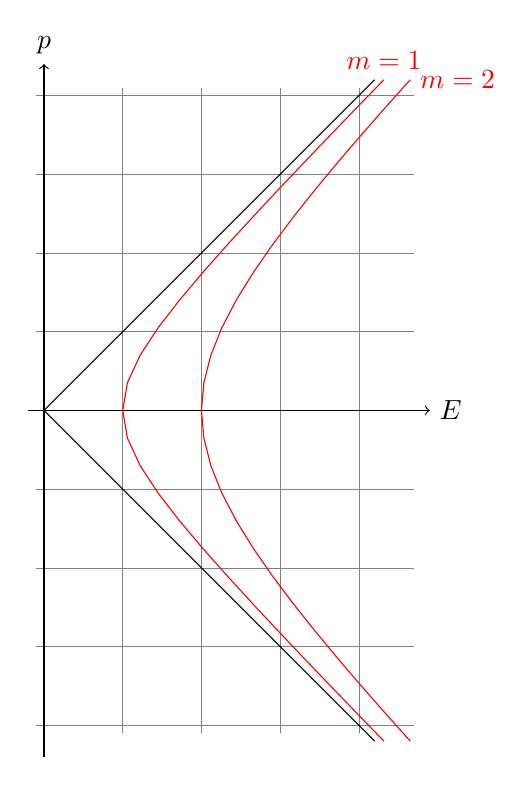
\begin{tikzpicture}[domain=-4.2:4.2]
  \draw [very thin,color=gray] (-0.1,-4.1) grid (4.7,4.1);
  \draw [->] (-0.2,0) -- (4.9,0) node[right] {$E$};
  \draw [->] (0,-4.4) -- (0,4.4) node[above] {$p$};
  \draw    plot ({sqrt(\x*\x)},\x);
  \draw [color=red]    plot ({sqrt(1+\x*\x)},\x)             node[above] {$m=1$};
  \draw [color=red]    plot ({sqrt(4+\x*\x)},\x)             node[right] {$m=2$};
\end{tikzpicture}
&
\textsf{In dit diagram zijn geen waarden bij de assen gezet maar is $m=1$ genomen. 
Omdat gelijke deeltjes en hun antideeltjes dezelfde massa hebben kunnen 
we hier ook de massa voor deze deeltjes in $\mathrm{eV}$ voor nemen. 
De schaal van de energie- en de impuls-as is direct gekoppeld aan de massa.}
\end{tabular}
\par\end{center}

\textsf{\caption{\label{fig:(p,E)-diagram}Het $\left(p,E\right)$-diagram}}
\end{figure}

Het is gebruikelijk om voor de eenheid van energie $\left[\mathrm{eV}\right]$
te gebruiken. Omdat $c=1$ hebben de grootheden $p$, $E$ en $m$
in dit geval dezelfde eenheid. De grootheden $m$ en $E$ zijn beide
scalair. De snelheid $v$ geeft de grootheid $p$ naast een grootte ook een richting 
en is dus een vectorgrootheid. De term $p^{2}$ kan worden ge\"interpreteerd
als de lengte in het kwadraat van de impulsvector (denk aan Pythagoras).
Voor het gemak gebruiken we in eerste instantie alleen een 1 dimensionale
ruimte. Nu kunnen we doen of $p$ een scalaire grootheid is.

Fotonen hebben geen rustmassa, voor fotonen geldt dus $E^{2}-p^{2}=\left(E-p\right)*\left(E+p\right)=0\mathrm{eV}$.
In het $\left(p,E\right)$-diagram in figuur \ref{fig:(p,E)-diagram}
liggen de toestanden van een foton dus altijd op rechte lijnen met
de wiskundige vergelijkingen $E=p$ of $E=-p$.

Deeltjes hebben daarentegen wel een rustmassa. Als $p=0$ wordt de $E$-as gesneden
bij $m$ omdat $E^{2}-0^{2}=m^{2}$. Andere toestanden van een deeltje
met massa $m$ liggen op een hyperbool door dit snijpunt. De hyperbool
nadert de lijnen $E=p$ en $E=-p$ asymptotisch.

\newpage{}

\section{Interacties in het (p,E)-diagram}

\begin{figure}[h]
\begin{center}
\begin{tabular}{ c c }
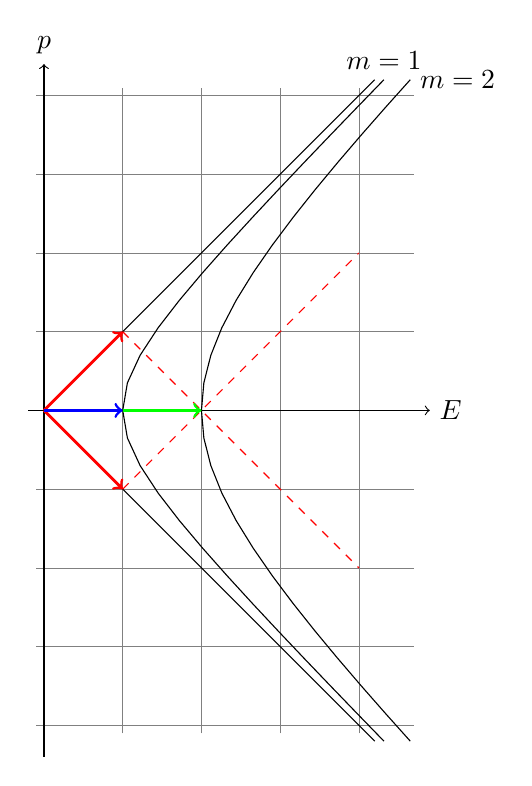
\begin{tikzpicture}[domain=-4.2:4.2]
  \draw [very thin,color=gray] (-0.1,-4.1) grid (4.7,4.1);
  \draw [->] (-0.2,0) -- (4.9,0) node[right] {$E$};
  \draw [->] (0,-4.4) -- (0,4.4) node[above] {$p$};
  \draw    plot ({sqrt(\x*\x)},\x);
  \draw    plot ({sqrt(1+\x*\x)},\x)             node[above] {$m=1$};
  \draw    plot ({sqrt(4+\x*\x)},\x)             node[right] {$m=2$};
  \draw [color=red,->, line width=1pt] (0,0) -- (1,1);
  \draw [color=red,->, line width=1pt] (0,0) -- (1,-1);
  \draw [color=red, dashed] (1,1) -- (4,-2);
  \draw [color=red, dashed] (1,-1) -- (4,2);
  \draw [color=blue,->, line width=1pt] (0,0) -- (1,0);
  \draw [color=green,->, line width=1pt] (1,0) -- (2,0);
\end{tikzpicture}
&
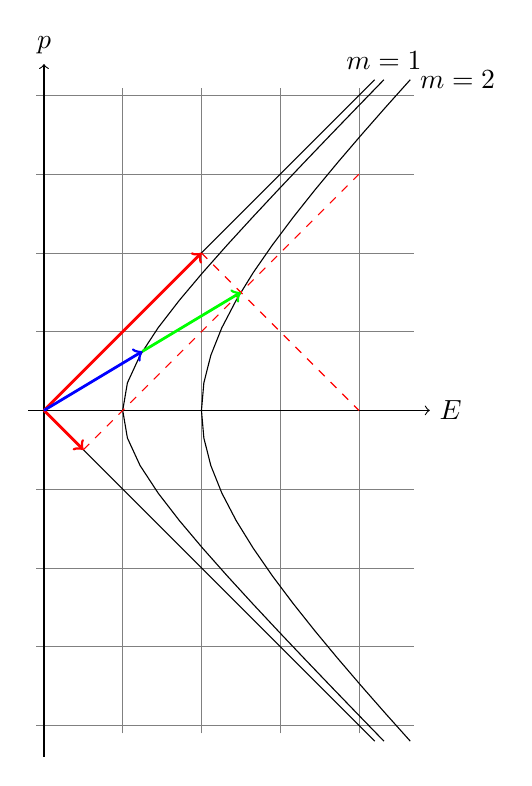
\begin{tikzpicture}[domain=-4.2:4.2]
  \draw [very thin,color=gray] (-0.1,-4.1) grid (4.7,4.1);
  \draw [->] (-0.2,0) -- (4.9,0) node[right] {$E$};
  \draw [->] (0,-4.4) -- (0,4.4) node[above] {$p$};
  \draw    plot ({sqrt(\x*\x)},\x);
  \draw    plot ({sqrt(1+\x*\x)},\x)             node[above] {$m=1$};
  \draw    plot ({sqrt(4+\x*\x)},\x)             node[right] {$m=2$};
  \draw [color=red,->, line width=1pt] (0,0) -- (2,2);
  \draw [color=red,->, line width=1pt] (0,0) -- (.5,-.5);
  \draw [color=red, dashed] (2,2) -- (4,0);
  \draw [color=red, dashed] (.5,-.5) -- (4,3);
  \draw [color=blue,->, line width=1pt] (0,0) -- (1.25,0.75);
  \draw [color=green,->, line width=1pt] (1.25,0.75) -- (2.5,1.5);
\end{tikzpicture}
\end{tabular}
\par\end{center}
\textsf{Door de toestandvectoren van beide fotonen op te tellen is de begintoestand van het systeem te bepalen (rood / parallellogrammethode). Er is precies voldoende energie voor de creatie van een deeltje (blauw) en een anti-deeltje (groen) in de eindtoestand, beide met een massa 1 (kop-staartmethode).
\caption{\label{fig:voldoende}De creatie van een deeltje en een antideeltje door de interactie van twee fotonen met een minimale energie in het $\left(p,E\right)$-diagram}}

\end{figure}

Zoals opgemerkt mogen we bij 1 dimensionale botsingen $p$ als scalair
beschouwen. Een mogelijke interactie, waarbij twee gamma fotonen (met
rustmassa $m=0\mathrm{eV}$) een electron en een positron cre\"eren,
is te schrijven als:

\begin{equation}
\gamma+\gamma\rightarrow e^{-}+\bar{e}^{+}
\end{equation}

In het totaal wordt er een rustmassa van $2*0.510998928(11)\mathrm{MeV}$
voor het elektron en het positron gecre\"eerd. Bij een minimale energie
(ten op zichte van een waarnemer) is de impuls na de interactie $0\mathrm{MeV}$.
Volgens de wet van behoud van impuls is de impuls voor de interactie
ook $0\mathrm{MeV}$. De impuls van beide fotonen is dus even groot
en tegengesteld. Voor fotonen geldt: $E=\pm p$ zodat de energie voor
beide fotonen hetzelfde moet zijn. De minimale energie voor ieder
foton is dus $0.510998928(11)\mathrm{MeV}$.

In dit voorbeeld hebben beide fotonen een evengrote tegengestelde
impuls. Als fotonen langs dezelfde lijn naar elkaar bewegen, hoeft
dit echter niet altijd zo te zijn. Bij het GZK-effect treden er interacties
met de kosmische achtergrondstraling (CMB, Cosmic Microwave Background)
op. De energie van deze CMB fotonen is veel lager. Bijgevolg moet
de energie van het andere foton veel hoger zijn. Nu is de som van
de impulsen geen $0\mathrm{MeV}$. De (energie, impuls) toestand van het
elektron en het anti-elektron kunnen nu grafisch worden bepaald.


Zoals in figuur \ref{fig:voldoende} te zien is, kunnen de toestanden van beide fotonen met twee $\left(p, 
E\right)$-vectoren worden beschreven. Als we deze vectoren vectorieel optellen
vinden we de toestandsvector voor het systeem van beide fotonen. Omdat
de wet van behoud van energie en de wet van behoud van impuls voor
deze waarnemer blijft gelden, is dit ook de toestandsvector voor het
elektron en het anti-elektron. De toestanden van beide deeltjes liggen
op een hyperbool door de rustmassa van beide deeltjes. 


Een overschot aan energie verandert het diagram, het deeltje en het anti-deeltje krijgen nu ook een extra impuls. Deze diagrammen zijn te zien in \ref{fig:overschot}


\begin{figure}[h]
\begin{center}
\begin{tabular}{ c c }
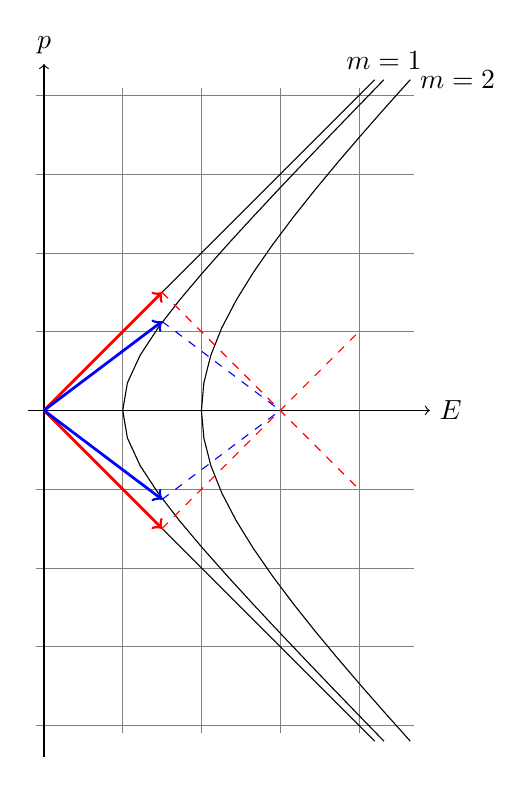
\begin{tikzpicture}[domain=-4.2:4.2]
  \draw [very thin,color=gray] (-0.1,-4.1) grid (4.7,4.1);
  \draw [->] (-0.2,0) -- (4.9,0) node[right] {$E$};
  \draw [->] (0,-4.4) -- (0,4.4) node[above] {$p$};
  \draw    plot ({sqrt(\x*\x)},\x);
  \draw    plot ({sqrt(1+\x*\x)},\x)             node[above] {$m=1$};
  \draw    plot ({sqrt(4+\x*\x)},\x)             node[right] {$m=2$};
  \draw [color=red,->, line width=1pt] (0,0) -- (1.5,1.5);
  \draw [color=red,->, line width=1pt] (0,0) -- (1.5,-1.5);
  \draw [color=red, dashed] (1.5,1.5) -- (4,-1);
  \draw [color=red, dashed] (1.5,-1.5) -- (4,1);
  \draw [color=blue,->, line width=1pt] (0,0) -- (1.5,1.13);
  \draw [color=blue,->, line width=1pt] (0,0) -- (1.5,-1.13);
  \draw [color=blue, dashed] (1.5,1.13) -- (3,0);
  \draw [color=blue, dashed] (1.5,-1.13) -- (3,0);
\end{tikzpicture}
&
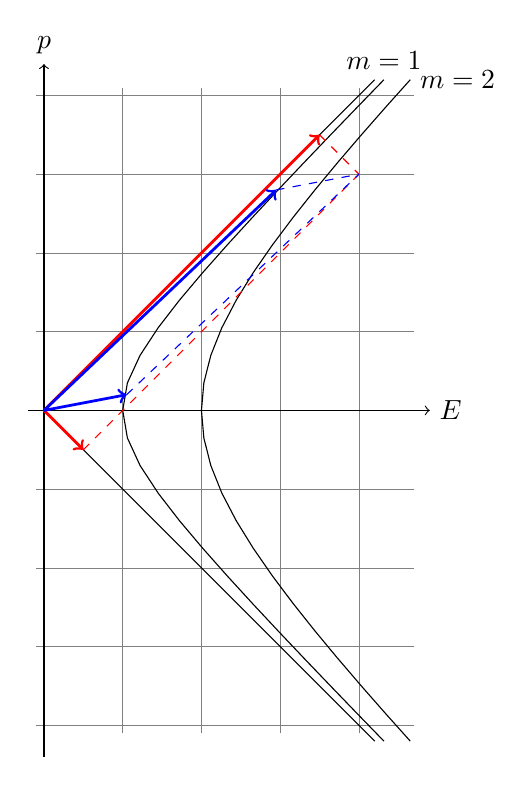
\begin{tikzpicture}[domain=-4.2:4.2]
  \draw [very thin,color=gray] (-0.1,-4.1) grid (4.7,4.1);
  \draw [->] (-0.2,0) -- (4.9,0) node[right] {$E$};
  \draw [->] (0,-4.4) -- (0,4.4) node[above] {$p$};
  \draw    plot ({sqrt(\x*\x)},\x);
  \draw    plot ({sqrt(1+\x*\x)},\x)             node[above] {$m=1$};
  \draw    plot ({sqrt(4+\x*\x)},\x)             node[right] {$m=2$};
  \draw [color=red,->, line width=1pt] (0,0) -- (3.5,3.5);
  \draw [color=red,->, line width=1pt] (0,0) -- (.5,-.5);
  \draw [color=red, dashed] (3.5,3.5) -- (4,3);
  \draw [color=red, dashed] (.5,-.5) -- (4,3);
  \draw [color=blue,->, line width=1pt] (0,0) -- (2.95,2.8);
  \draw [color=blue,->, line width=1pt] (0,0) -- (1.05,0.2);
  \draw [color=blue, dashed] (2.95,2.8) -- (4,3);
  \draw [color=blue, dashed] (1.05,0.2) -- (4,3);
\end{tikzpicture}
\end{tabular}
\par\end{center}
\textsf{Ook nu zijn de toestandsvectoren van beide fotonen opgeteld om de begintoestand van het systeem te bepalen (rood / paralellogrammethode). Er is ruim voldoende energie voor de creatie van een deeltje en een anti-deeltje in de eindtoestand. (blauw / paralellogrammethode). Een deel van de energie wordt omgezet in extra bewegingsenergie. De impuls van beide deeltjes verandert.
\caption{\label{fig:overschot}Een foton / foton interactie met een energieoverschot in het $\left(p,E\right)$-diagram}}
\end{figure}


\newpage{}

\section{Interacties in 3 dimensies}

Tot nu toe zijn we uitgegaan van een 1 dimensionale ruimte. Uiteindelijk willen we naar een ruimte met 3 dimensies. Bij interacties in de ruimte wordt de waarnemer meestal in het centrum van de interactie geplaatst. In de figuren \ref{fig:voldoende} en \ref{fig:overschot} is dit altijd het linkerdiagram. In de rechterdiagrammen zie je de interactie als het ware voorbijsnellen. Eigenlijk zijn er impulsveraanderingen in de richting van de interactie en loodrecht op de richting van de interactie. Hiermee zijn alle ruimtelijke interacties te beschrijven.

Het $(p,E)$-diagram krijgt nu een extra as loodrecht op de $p$-as. De toestanden liggen nu niet meer op een hyperbool maar op een hyperbolisch omwentelings lichaam. De doorneden in $\left(p_{//},p_{\perp}\right)$-vlakken zijn allen cirkelvormig. De totale impuls van het systeem is in fig. \ref{fig:overschot} af te lezen. Deze impuls is altijd in de $p_{//}$-richting. Bij de creatie van een deeltje en een anti-deeltje is de straal van het hyperbolisch omwentingslichaam in fig. \ref{fig:overschot} te vinden bij de energie van het deeltje of de halve energie van het systeem. Voor de deeltjes geldt $p_{1,//}=p_{2,//}=p_{systeem}/2$.

\begin{figure}[h]
\begin{center}

\begin{tabular}{ c c }
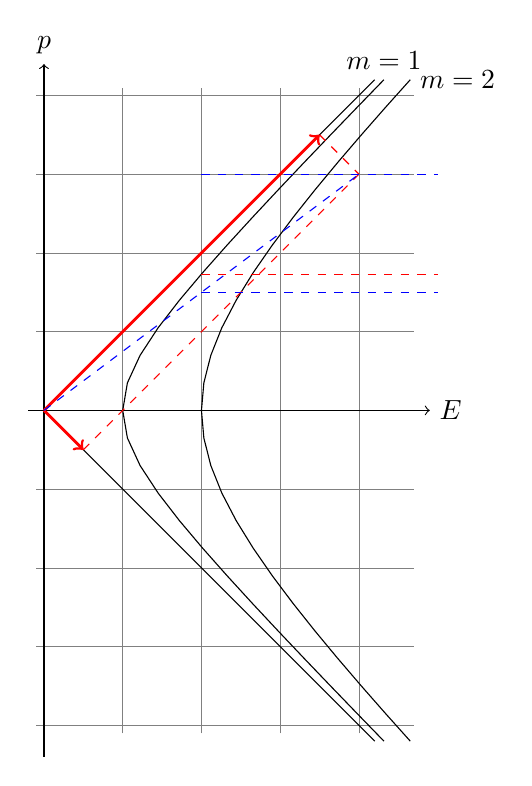
\begin{tikzpicture}[domain=-4.2:4.2]
  \draw [very thin,color=gray] (-0.1,-4.1) grid (4.7,4.1);
  \draw [->] (-0.2,0) -- (4.9,0) node[right] {$E$};
  \draw [->] (0,-4.4) -- (0,4.4) node[above] {$p$};
  \draw    plot ({sqrt(\x*\x)},\x);
  \draw    plot ({sqrt(1+\x*\x)},\x)             node[above] {$m=1$};
  \draw    plot ({sqrt(4+\x*\x)},\x)             node[right] {$m=2$};
  \draw [color=red,->, line width=1pt] (0,0) -- (3.5,3.5);
  \draw [color=red,->, line width=1pt] (0,0) -- (.5,-.5);
  \draw [color=red, dashed] (3.5,3.5) -- (4,3);
  \draw [color=red, dashed] (2,1.73) -- (5,1.73);
  \draw [color=red, dashed] (.5,-.5) -- (4,3);
  \draw [color=blue, dashed] (0,0) -- (4,3);
  \draw [color=blue, dashed] (2,1.5) -- (5,1.5);
  \draw [color=blue, dashed] (2,3) -- (5,3);
\end{tikzpicture}
&
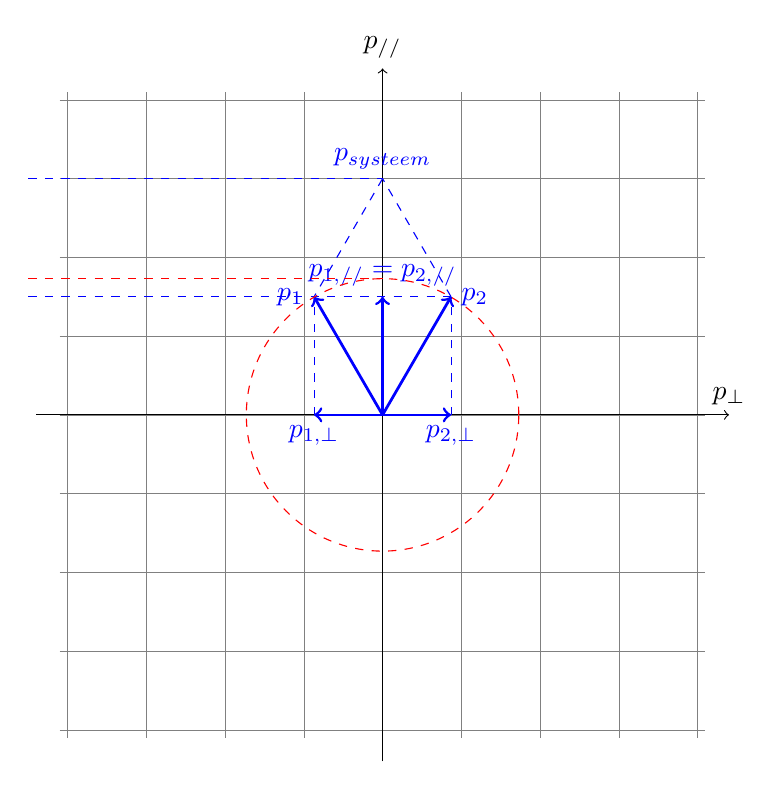
\begin{tikzpicture}[domain=-4.2:4.2]
  \draw [very thin,color=gray] (-4.1,-4.1) grid (4.1,4.1);
  \draw [->] (-4.4,0) -- (4.4,0) node[above] {$p_{\perp}$};
  \draw [->] (0,-4.4) -- (0,4.4) node[above] {$p_{//}$};
  \draw [color=blue, ->, line width=1pt] (-0.,0) -- (0,1.5) node[above] {$p_{1,//}=p_{2,//}$};
  \draw [color=blue, ->, line width=1pt] (0.,0) -- (0.87,1.5) node[right] {$p_{2}$};
  \draw [color=blue, ->, line width=1pt] (0.,0) -- (-0.87,1.5) node[left] {$p_{1}$};
  \draw [color=blue, dashed] (0.87,1.5) -- (0.,3) node[above] {$p_{systeem}$};
  \draw [color=blue, dashed] (0.,3) -- (-0.87,1.5);
  \draw [color=blue, dashed] (0.87,0) -- (0.87,1.5);
  \draw [color=blue, dashed] (-0.87,0) -- (-0.87,1.5);
  \draw [color=blue, ->, line width=1pt] (-0.,0) -- (0.87,0) node[below] {$p_{2,\perp}$};
  \draw [color=blue, ->, line width=1pt] (-0.,0) -- (-0.87,0) node[below] {$p_{1,\perp}$};
  \draw [color=blue, dashed] (-4.5,1.5) -- (0.87,1.5);
  \draw [color=blue, dashed] (-4.5,3) -- (0,3);
  \draw [color=red, dashed] (-4.5,1.73) -- (0,1.73);
  \draw [color=red, dashed] (0,0) circle (1.73cm);
\end{tikzpicture}
\end{tabular}
\par\end{center}
\textsf{Het linkerdiagram komt uit \ref{fig:overschot}. Het rechterdiagram is een doorsnede bij $E=E_{systeem}/2$. In de ruimtelijke situatie bestaan $p_{1}$ en $p_{2}$ beide uit een component in de richting van de impuls van het systeem en een loodrechte component. De totale impuls van de deeltjes raakt (de doorsnede van) het hyperbolisch omwentelingslichaam zodat $p_{1,\perp}=-p_{2,\perp}$.
\caption{\label{fig:doorsnede}De doorsnede van het $(p,E)$ hyperbolisch omwentingslichaam bij $E_{deeltje}$ in het $\left(p_{//},p_{\perp}\right)$-diagram}}
\end{figure}

De hoek waaronder het deeltje en het anti-deeltje volgens deze waarnemer wegschieten is direct in fig. \ref{fig:doorsnede} te meten. In dit geval schieten het deeltje en het anti-deeltje onder hoeken van $30^{\mathrm{o}}$ weg, zodat de som van de loodrechte impulsen $0\mathrm{eV}$ blijft. 

Deze methode werkt alleen als de massa van beide deeltje gelijk is. Als de massa verschilt wordt de waarnemer verplaatst omdat afstanden, tijd, massa en daarmee snelheid en impuls geen invarianten zijn. We kiezen eerst een zo eerlijk mogelijk waarnemer. De waarnemer wordt in het centrum van de interactie geplaatst, dit noemen we "botsingscentraal". De som van alle impulsen van het systeem is volgens deze waarnemer $0\mathrm{eV}$. In figuur \ref{fig:waarnemers} is te zien hoe we de waarnemer met het $(p,E)$-diagram kunnen verplaatsen.

\begin{figure}[h]
\begin{center}
\begin{tabular}{ c c }
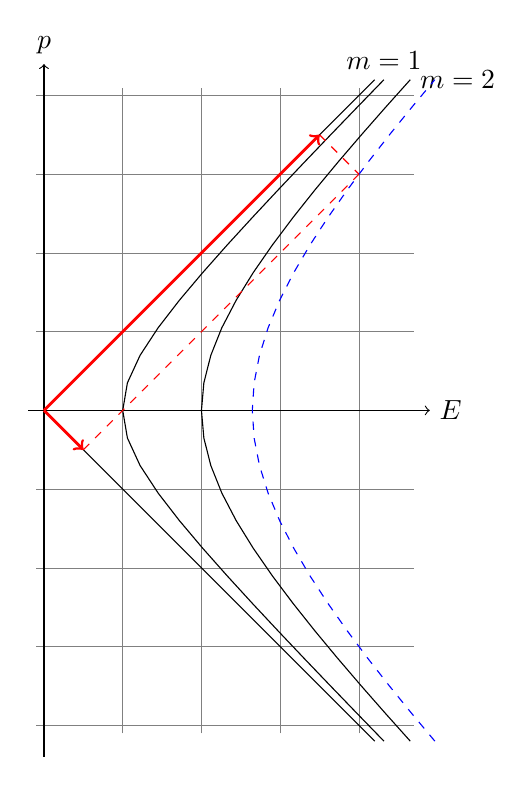
\begin{tikzpicture}[domain=-4.2:4.2]
  \draw [very thin,color=gray] (-0.1,-4.1) grid (4.7,4.1);
  \draw [->] (-0.2,0) -- (4.9,0) node[right] {$E$};
  \draw [->] (0,-4.4) -- (0,4.4) node[above] {$p$};
  \draw    plot ({sqrt(\x*\x)},\x);
  \draw    plot ({sqrt(1+\x*\x)},\x)             node[above] {$m=1$};
  \draw    plot ({sqrt(4+\x*\x)},\x)             node[right] {$m=2$};
  \draw [color=blue, dashed] plot ({sqrt(7+\x*\x)},\x);
  \draw [color=red,->, line width=1pt] (0,0) -- (3.5,3.5);
  \draw [color=red,->, line width=1pt] (0,0) -- (.5,-.5);
  \draw [color=red, dashed] (3.5,3.5) -- (4,3);
  \draw [color=red, dashed] (.5,-.5) -- (4,3);
\end{tikzpicture}
&
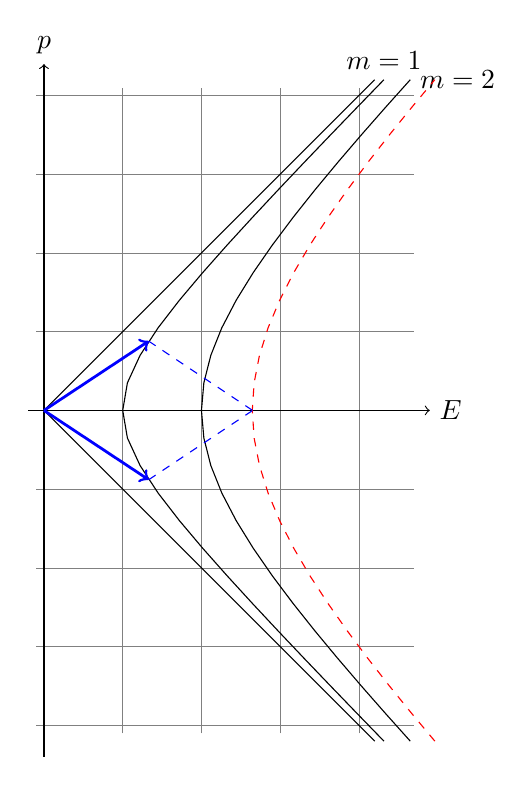
\begin{tikzpicture}[domain=-4.2:4.2]
  \draw [very thin,color=gray] (-0.1,-4.1) grid (4.7,4.1);
  \draw [->] (-0.2,0) -- (4.9,0) node[right] {$E$};
  \draw [->] (0,-4.4) -- (0,4.4) node[above] {$p$};
  \draw    plot ({sqrt(\x*\x)},\x);
  \draw    plot ({sqrt(1+\x*\x)},\x)             node[above] {$m=1$};
  \draw    plot ({sqrt(4+\x*\x)},\x)             node[right] {$m=2$};
  \draw [color=red, dashed]   plot ({sqrt(7+\x*\x)},\x);
  \draw [color=blue,->, line width=1pt] (0,0) -- (1.33,0.88);
  \draw [color=blue,->, line width=1pt] (0,0) -- (1.33,-0.88);
  \draw [color=blue, dashed] (1.33,0.88) -- (2.65,0);
  \draw [color=blue, dashed] (1.33,-0.88) -- (2.65,0);
\end{tikzpicture}
\end{tabular}
\par\end{center}
\textsf{In het linkerdiagram wordt de hyperbool met toestanden van het systeem met beide fotonen bepaald. Het parallellogram raakt de hyperbool volgens een waarnemer in het laboratorium. Het linkerdiagram wordt waargenomen  door een laboratoriumwaarnemer. In het rechterdiagram plaatsen we een waarnemer in het centrum van de botsing (botsingscentraal). Volgens deze waarnemer schieten de deeltjes even snel in tegengestelde richtingen weg. Dit kan dus in \textit{alle} tegengestelde richtingen.
\caption{\label{fig:waarnemers}Twee waarnemers in het $\left(p,E\right)$-diagram}}
\end{figure}

\newpage{}

\begin{figure}[h]
\begin{center}
\begin{tabular}{ c c }
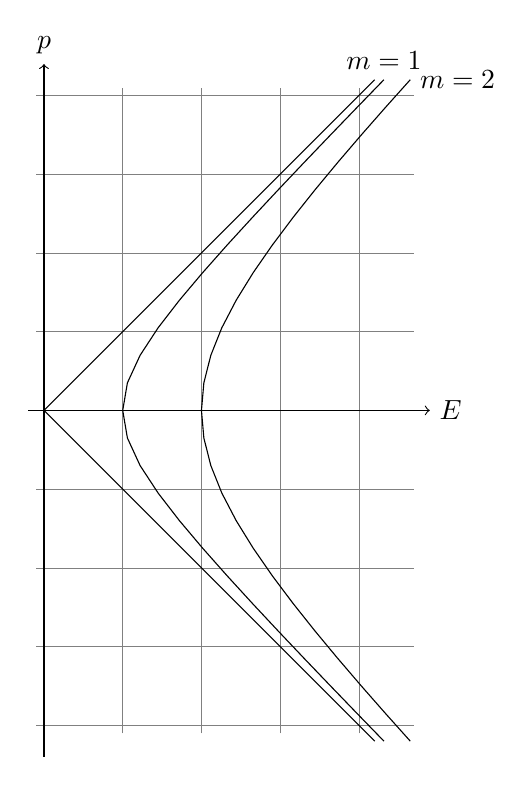
\begin{tikzpicture}[domain=-4.2:4.2]
  \draw [very thin,color=gray] (-0.1,-4.1) grid (4.7,4.1);
  \draw [->] (-0.2,0) -- (4.9,0) node[right] {$E$};
  \draw [->] (0,-4.4) -- (0,4.4) node[above] {$p$};
  \draw    plot ({sqrt(\x*\x)},\x);
  \draw    plot ({sqrt(1+\x*\x)},\x)             node[above] {$m=1$};
  \draw    plot ({sqrt(4+\x*\x)},\x)             node[right] {$m=2$};
\end{tikzpicture}
&
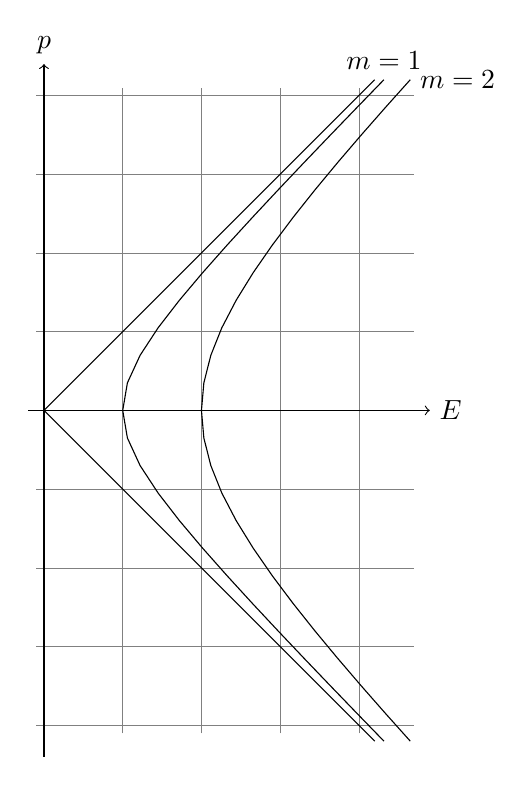
\begin{tikzpicture}[domain=-4.2:4.2]
  \draw [very thin,color=gray] (-0.1,-4.1) grid (4.7,4.1);
  \draw [->] (-0.2,0) -- (4.9,0) node[right] {$E$};
  \draw [->] (0,-4.4) -- (0,4.4) node[above] {$p$};
  \draw    plot ({sqrt(\x*\x)},\x);
  \draw    plot ({sqrt(1+\x*\x)},\x)             node[above] {$m=1$};
  \draw    plot ({sqrt(4+\x*\x)},\x)             node[right] {$m=2$};
\end{tikzpicture}

\tabularnewline

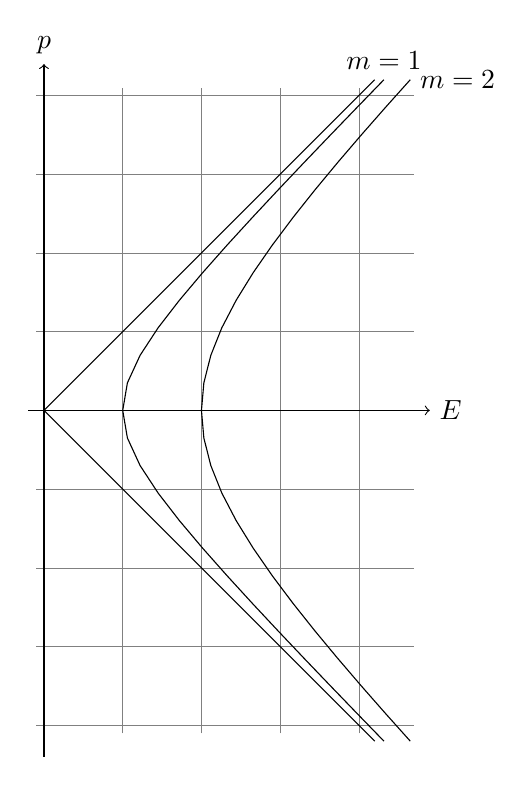
\begin{tikzpicture}[domain=-4.2:4.2]
  \draw [very thin,color=gray] (-0.1,-4.1) grid (4.7,4.1);
  \draw [->] (-0.2,0) -- (4.9,0) node[right] {$E$};
  \draw [->] (0,-4.4) -- (0,4.4) node[above] {$p$};
  \draw    plot ({sqrt(\x*\x)},\x);
  \draw    plot ({sqrt(1+\x*\x)},\x)             node[above] {$m=1$};
  \draw    plot ({sqrt(4+\x*\x)},\x)             node[right] {$m=2$};
\end{tikzpicture}
&
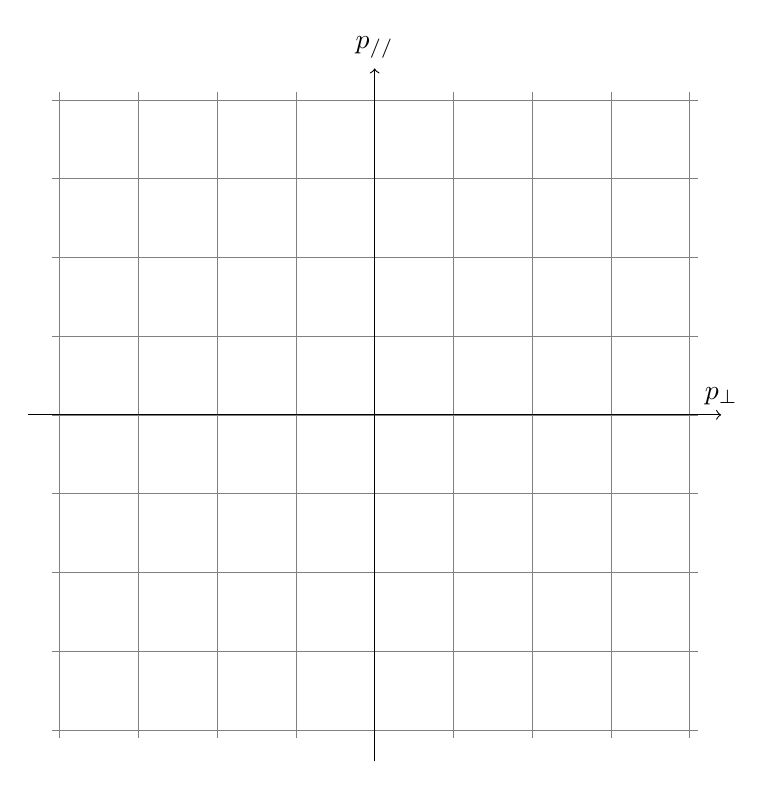
\begin{tikzpicture}[domain=-4.2:4.2]
  \draw [very thin,color=gray] (-4.1,-4.1) grid (4.1,4.1);
  \draw [->] (-4.4,0) -- (4.4,0) node[above] {$p_{\perp}$};
  \draw [->] (0,-4.4) -- (0,4.4) node[above] {$p_{//}$};
\end{tikzpicture}
\end{tabular}
\par\end{center}
\end{figure}


\end{document}
